%==========================================================================
%HTTP/2
%2015/04/08 (rumeda@mikilab.doshisha.ac.jp)
%==========================================================================

\documentclass[a4j,9pt,twocolumn]{jsarticle}
\usepackage{mlm2.0}
\usepackage{epsf}
\pagestyle{plain}


\begin{document}
\twocolumn[
%---------------------------------------------------------------------------
% ヘッダ    書式:\beginheader{回}{年}{月}
%---------------------------------------------------------------------------
\beginheader{161}{2015}{4}


%---------------------------------------------------------------------------
% 発表題目    書式:\title{日本語}{英語} 「\\」で改行できます
%---------------------------------------------------------------------------
\title%
{HTTP/2}%


%---------------------------------------------------------------------------
% 著者名      書式:\author{日本語著者名}{英語著者名}
%---------------------------------------------------------------------------
\author{梅田 玲旺,松井 健人,内村 祐之,市川 耀\\Reo UMEDA,Kento MATSUI,Yushi UCHIMURA,Hikaru ICHIKAWA}

%---------------------------------------------------------------------------


\endheader

%\begin{abstract}
%---------------------------------------------------------------------------
%Recently, a DVD attracts attention along with the image and the digitization of the sound. The standards of these DVD are complicated. So, in this paper, the standards of the DVD are summarized and the DVD of the next generation is refered. 
%---------------------------------------------------------------------------
%\end{abstract}
\vspace{3mm}
]

%---------------------------------------------------------------------------
% 本文
%---------------------------------------------------------------------------

\section{はじめに}
最近のWebサイトではWebサーバとブラウザ間でやり取りをしなければならないデータの量が増えてきている。そのためページ全体が表示されるのに遅くなる要因になってしまう。HTTP/1.1では複数のコネクションを同時に使いデータを早く送る方法が存在するがサーバやブラウザの負荷を増やしてしまい余計に遅くさせてしまう可能性がある。また、ダウンロードするのに時間のかかるHTTPのリクエストなどに対する応答が遅くなってしまい、先頭の応答が処理中であるため後続の応答まで全てブロックされるというHTTP/1.1の仕様もあり、コネクション数を増やしても効果が得られないことがある。

\section{HTTPの歴史}
 HTTPは1990年ごろ素粒子物理学の研究所であるCERNのティム・バーナーズ・リー氏がHTMLと共にCERN内の情報にアクセスするために設計をした。HTTP/0.9はテキストがメインの簡単なやり取りのみだったがその後1996年にHTTP/1.0の仕様が公開されContent-Typeのような各種ヘッダが追加され音楽や画像、動画などの様々なデータのやり取りに対応した。1999年に公開されたHTTP/1.1は複数のデータを効率よく転送するための持続的接続やプロキシの利用等を想定した仕様になっていた。持続的接続によってTCP接続を毎回行わずに繋いだままにして他のデータも通信していくことができる。また2000年からは日本では回線がADSLになりさらに今では光回線となり通信速度は速くなっていった。しかし回線が速くなったためにより多くのデータのやり取りが出来るようになり一つのページを構成する要素が多くなり、またデータ量が大きくなるなどしたためページサイズは増え続けていっている。よってHTTP/1.1で無駄になってしまっている部分を改良し効率的にする必要がある。



\section{HTTP/2の仕様}
\subsection{HTTP/2の特徴}
HTTP/2では実質的な転送速度を向上させることを目的としている。そのために通信路を仮想的に多重化して素早いレスポンスを実現しつつ,ヘッダのデータ圧縮で送信するデータを少なくしている。
いままでのHTTPと混在していくためにHTTP/1.1からHTTP/2の通信に移行するように際に、HTTP/2に対応しているかどうかを確認する。HTTP/2に未対応であればHTTP/1.1での通信を行うことで互換性を保っている。



\subsection{バイナリの使用}
HTTP/1.1のときはテキスト形式を使っていたがHTTP/2は高速化のためコマンドやパラメータの送信データを「フレーム」という形の決まったバイナリ形式のデータにまとめて送信するようになりフレームでHTTP/2はやり取りをするようになっている。そうすると小さな容量で転送ができテキストプロトコルとは違い空白の処理や大文字小文字など対応しなくてもよくなり間違いを少なくなり決まりきった形になっているため解析しやすくすることが出来る。フレームは以下Fig.1のようになっている。

\begin{figure}[h]
\centering
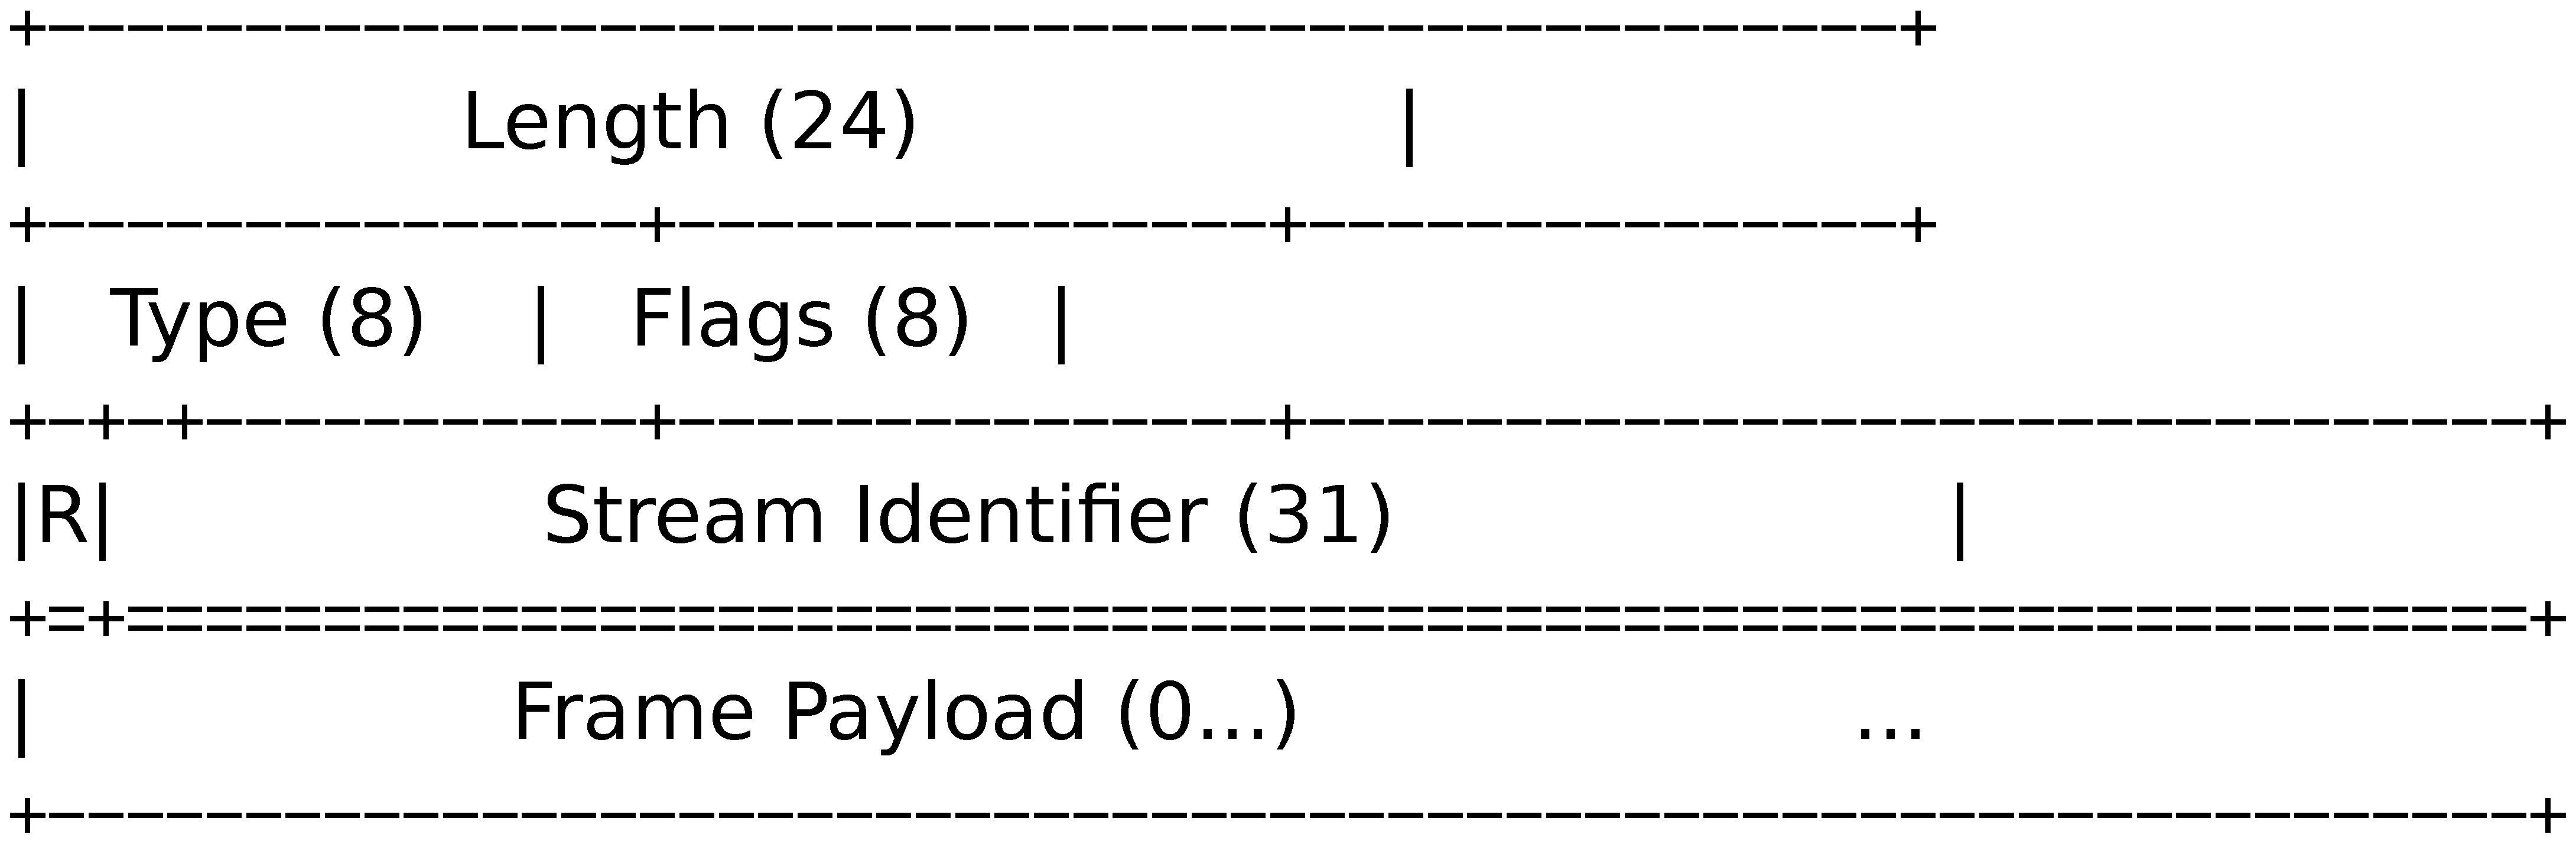
\includegraphics[width=80mm]{img/flame.eps}
\caption{HTTP/2のフレーム}
\end{figure}

Lengthが中身についての大きさでTypeはフレームのタイプを表しFlagsはフレームタイプのフラグのためにとられている。またRは定義されていない意味のない部分です。Stream IdentifierはストリームIDを表しています。その後は中身です。

\subsection{多重化}
コネクションを確立してまた「ストリーム」という仮想的な通信路を作りそれを使い双方向に「フレーム」を送受信する。
1つのコネクションで複数のストリームを作るとHTTP/1.1での複数のコネクションを使ったのと同等以上やり取りができるがHTTP/1.1では複数のコネクションを使用しやり取りをするがHTTP/2はコネクションが1つで済むためルーターやファイアウォール、プロキシサーバなどのネットワーク全体に対する負担が少なくなる。コネクションのイメージをFig.2に示す

\begin{figure}[h]
\centering
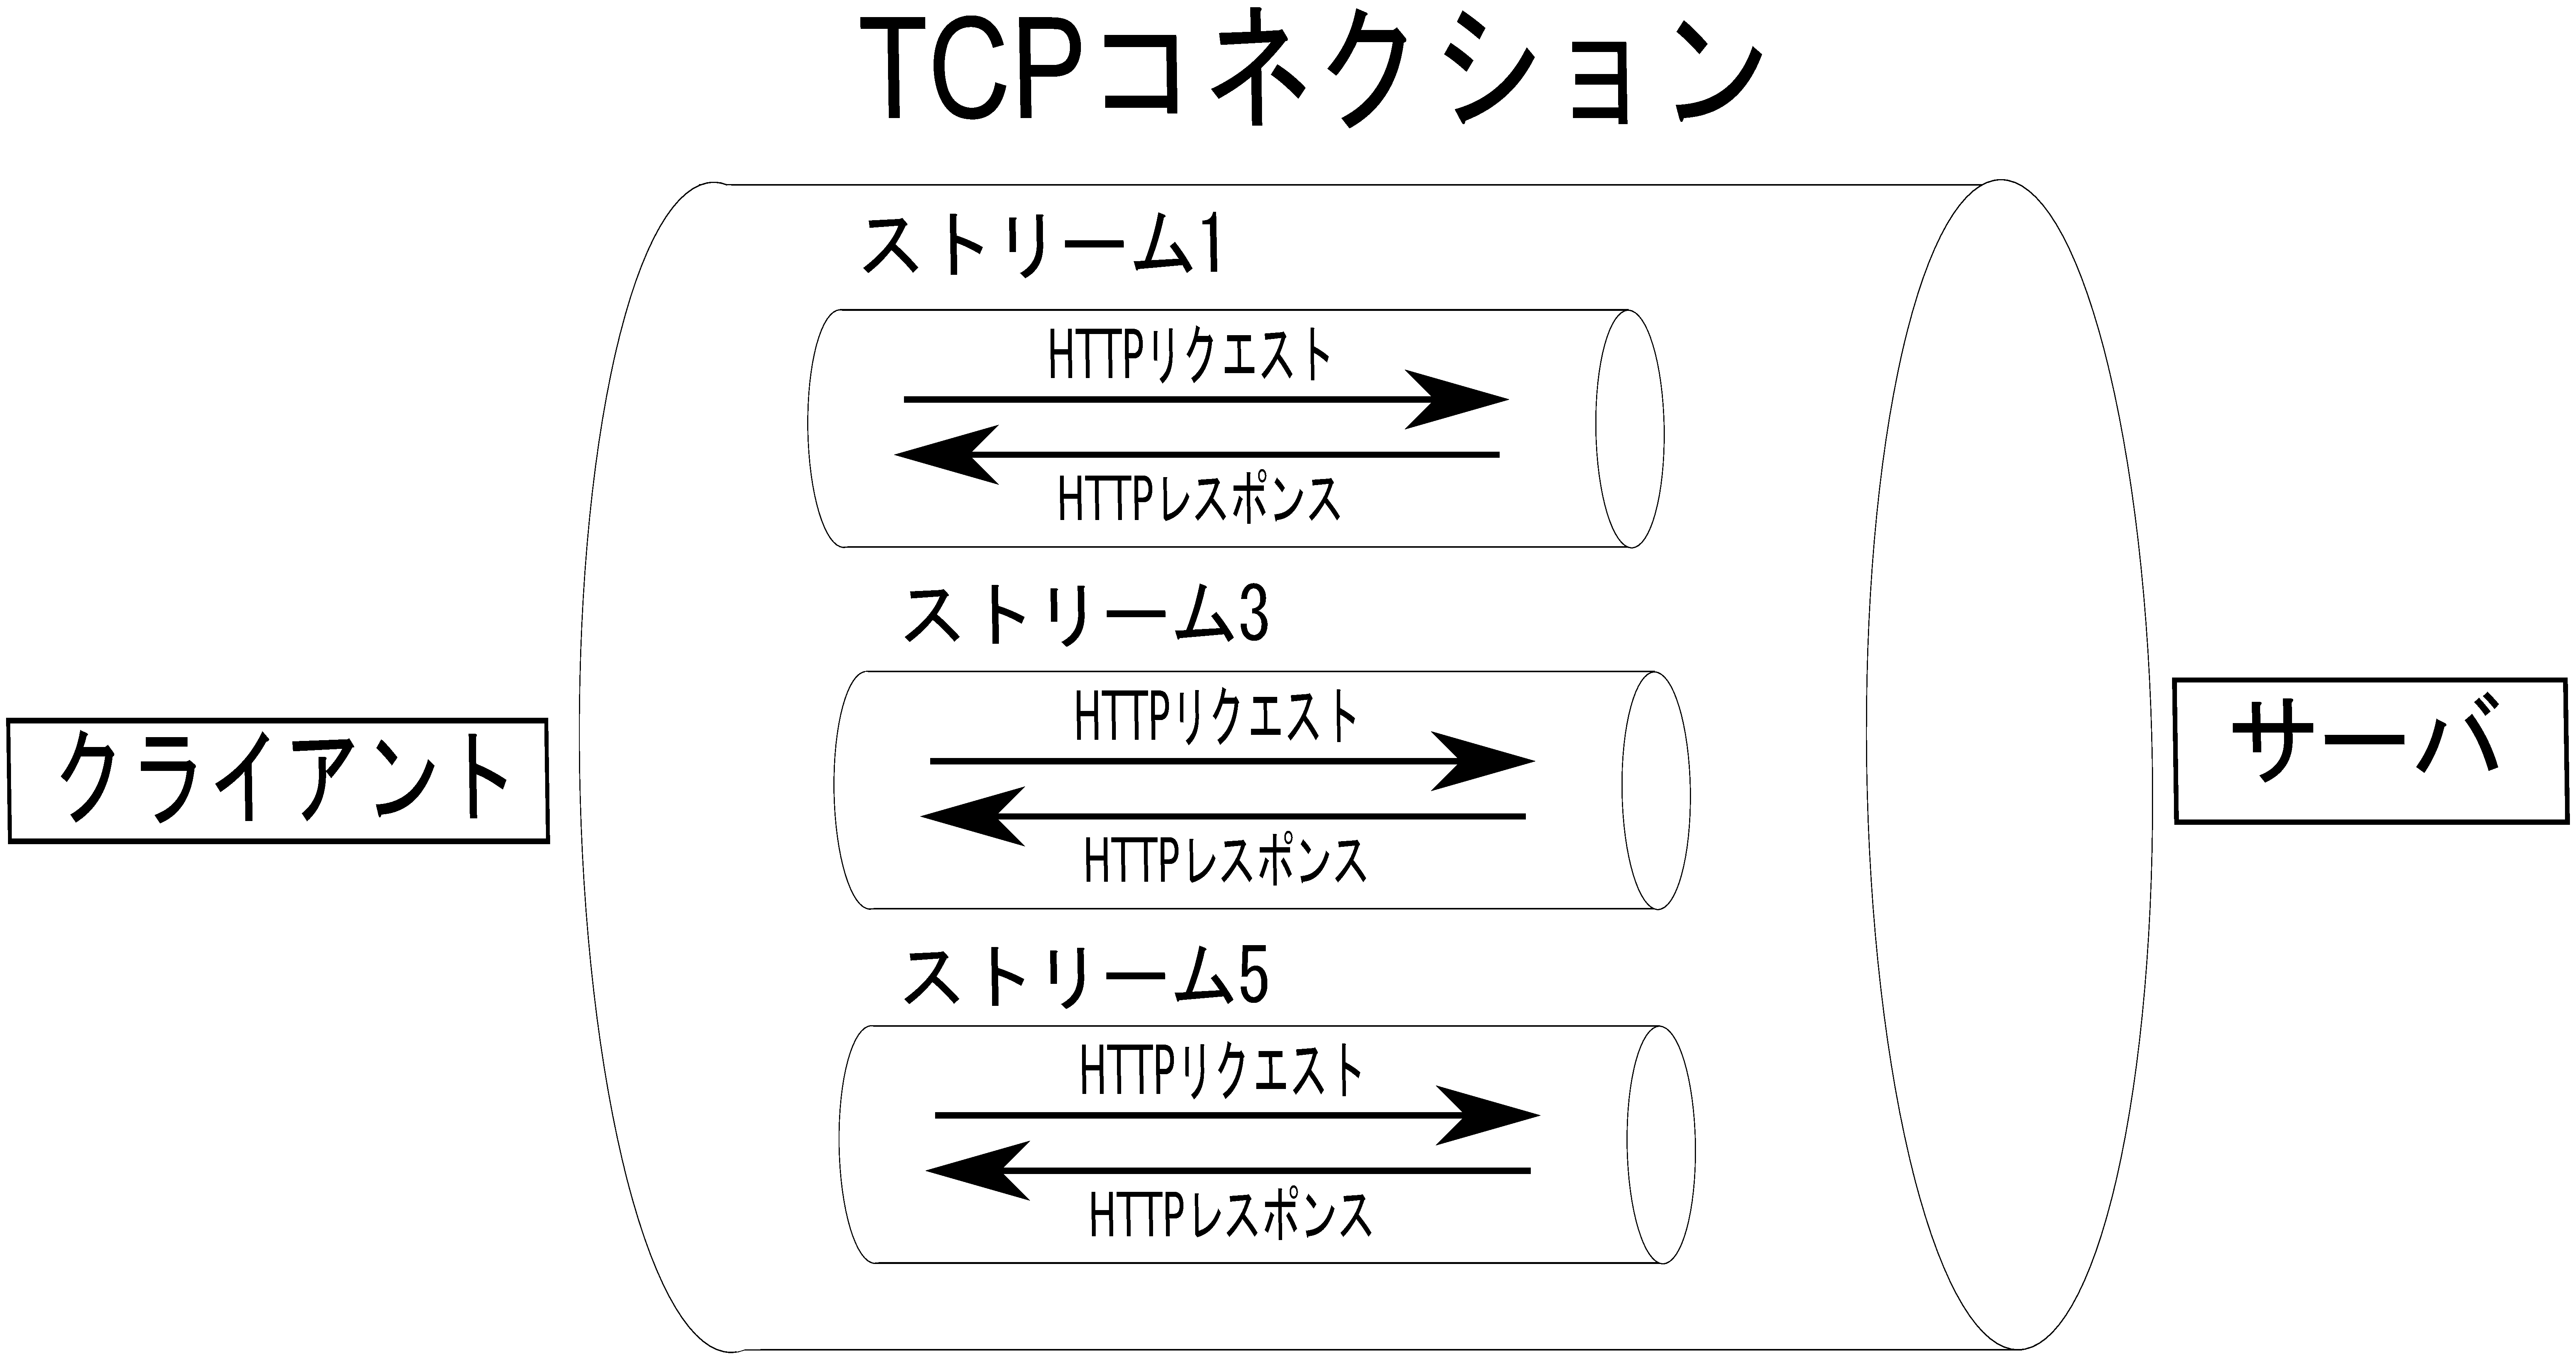
\includegraphics[width=80mm]{img/TCPco.eps}
\caption{HTTP/2のコネクションとストリーム}
\end{figure}

図のようにHTTP/1.1とは違いブラウザとサーバ間のコネクションは1つだけにしたほうが良いようになっている。
HTTP/1.1でも「パイプライン」機能を使えば、1つのコネクションで複数のリクエストを連続して送信することが可能だったが、その場合は、ブラウザに帰ってるレスポンスは送信したリクエスト順になる。だがHTTP/2のストリームではレスポンスの順番を変更できるので、例えばサーバ側の処理が重い場合は、それ以外の軽い処理のレスポンスを先に返す、といったことが可能になる。それをFig.3に示す。

\begin{figure}[h]
\centering
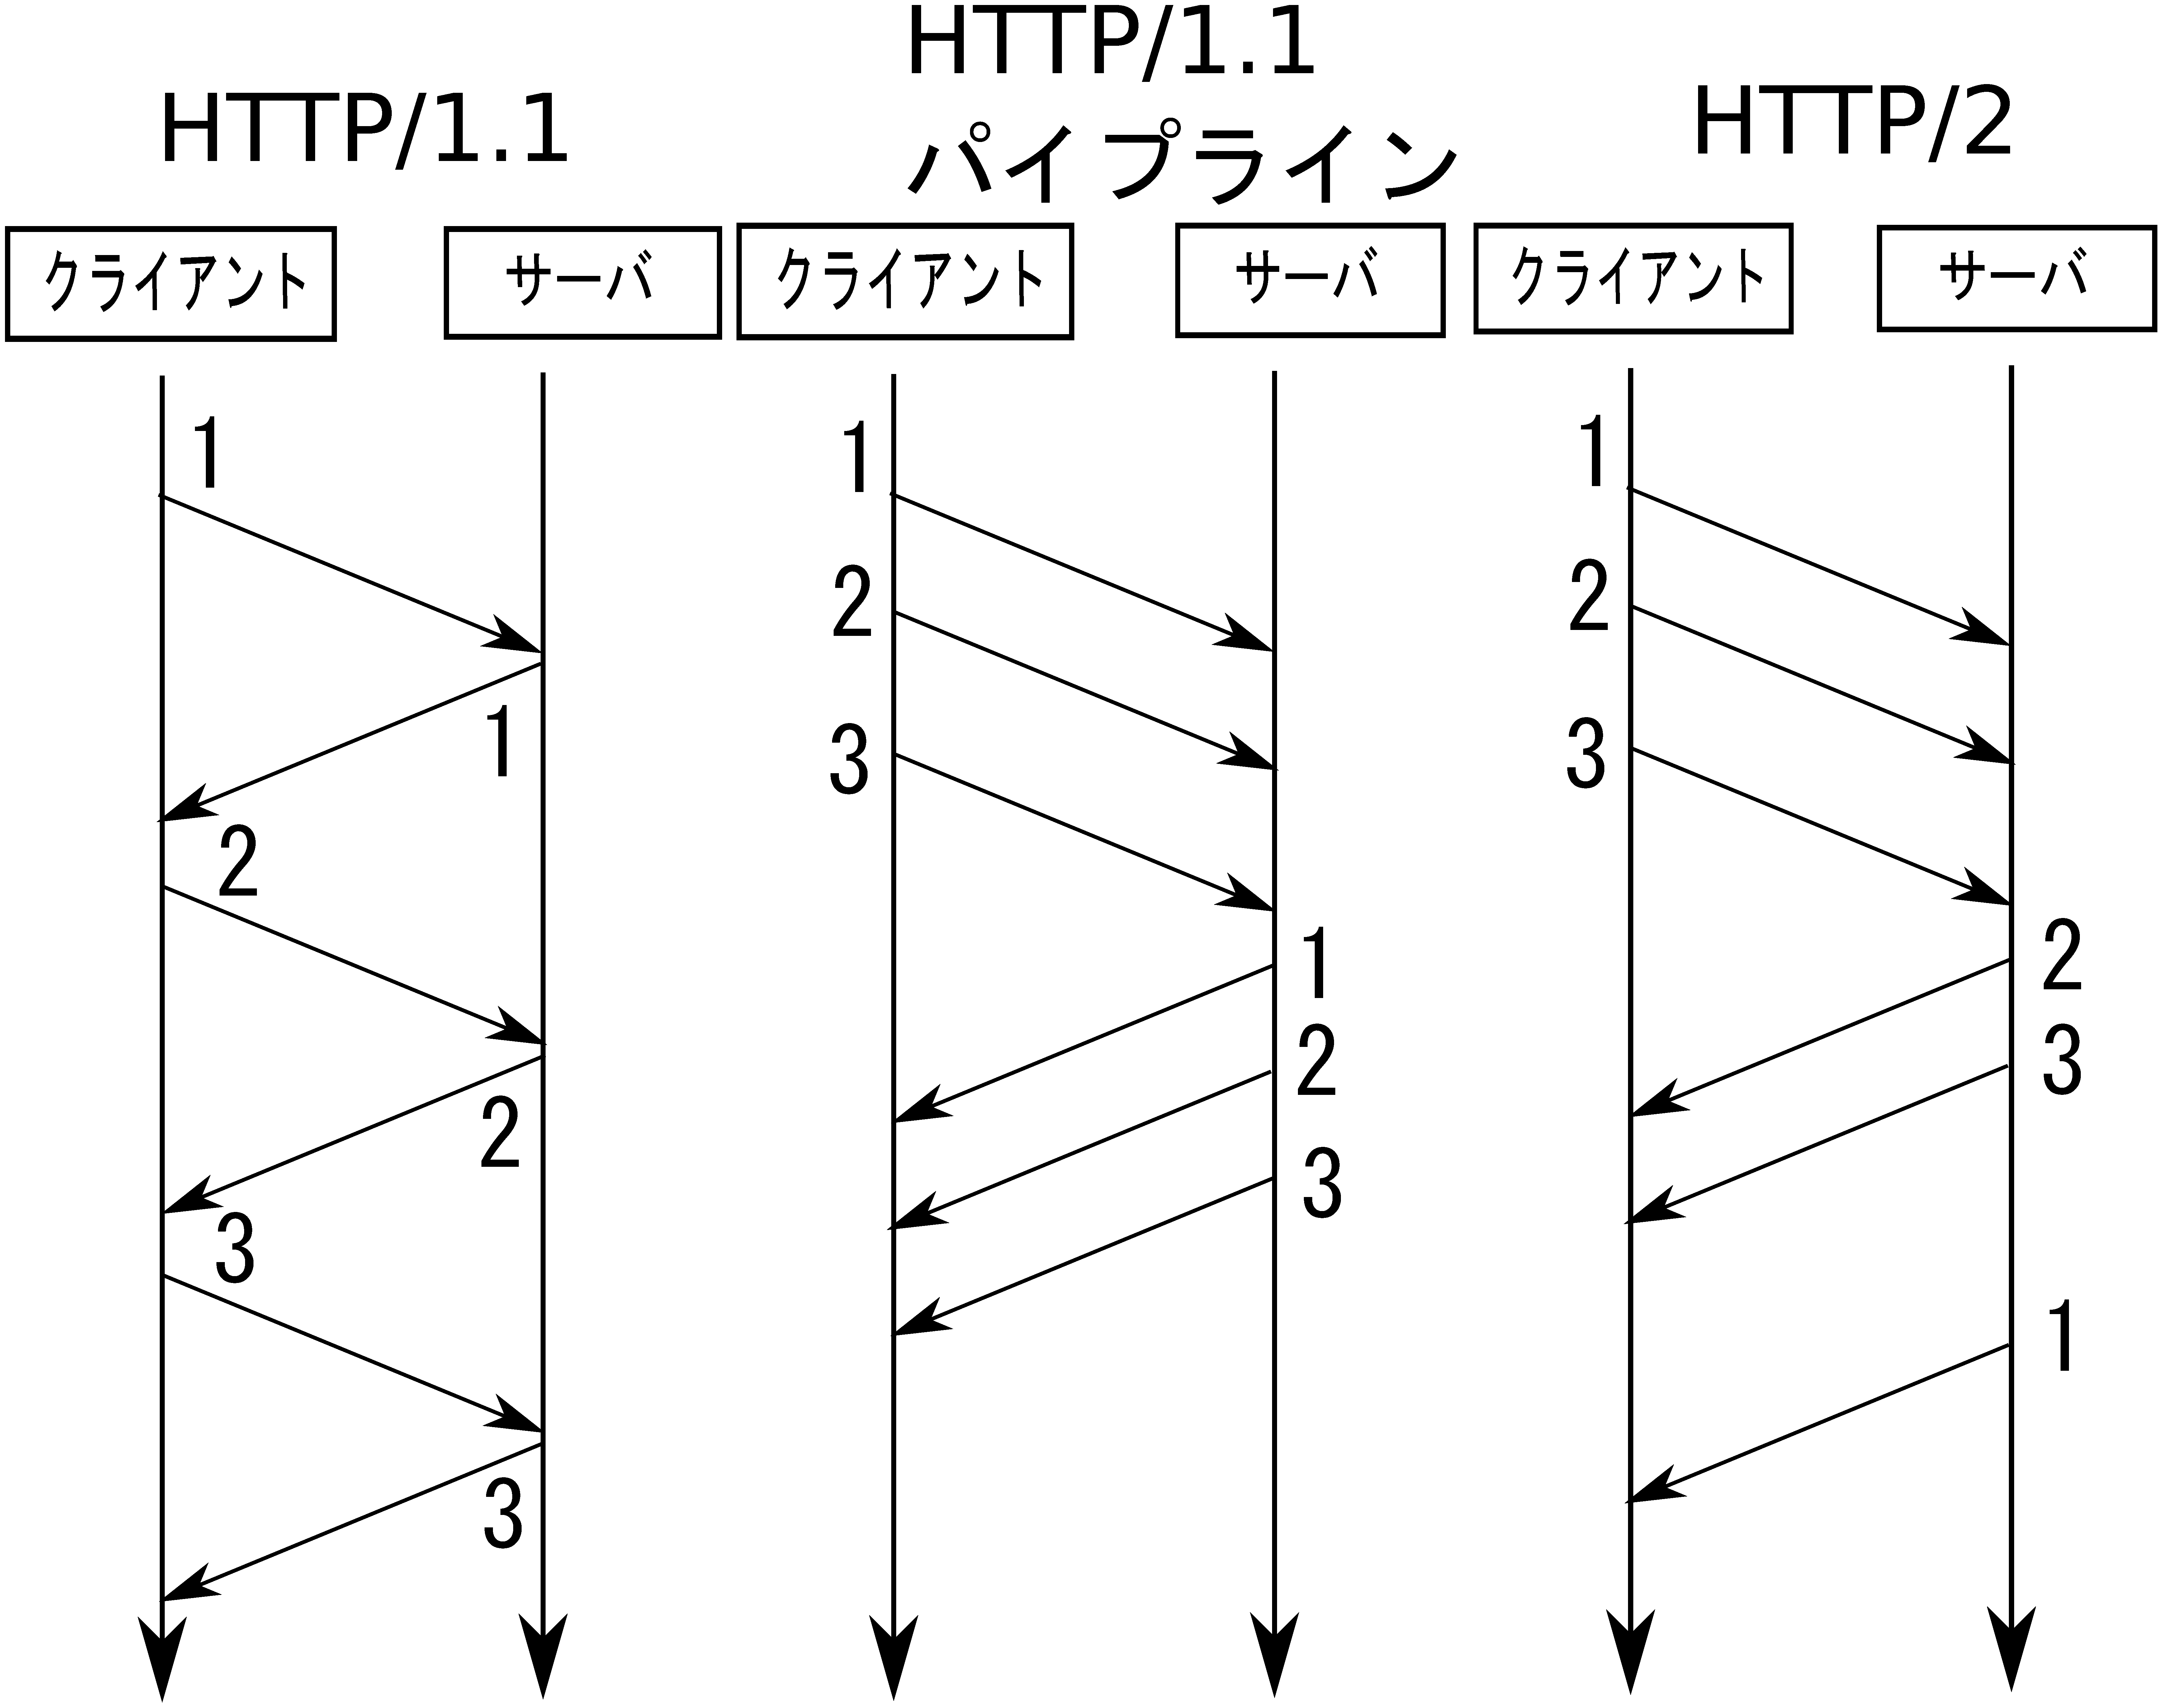
\includegraphics[width=80mm]{img/RR.eps}
\caption{HTTPのリクエストとレスポンス}
\end{figure}


ストリームには「優先度」を指定することもでき、ブラウザは後から優先度の高いリクエストを送って、その結果を先に返すようにサーバに対して要求できる優先度制御がある。例えば文字よりも表示するために時間のかかる画像を優先度を上げ先に送って貰うことができるようになる。
 HTTP/2では通信の状態を制御する機能として、「フロー制御」機能も用意されている。
一度に送信可能なデータ量を調整して受信側のバッファがあふれて容量不足になってしまうのを防いだり、逆に一度に送受信できるデータを大きく指定して、巨大なデータを効率よく送信させたりできる。HTTP/1.1ではTCP/IPのネットワーク機能を実現するために必要なTCPの機能に含まれるウィンドウ制御に依存していたが、HTTP/2ではWebサーバやブラウザがある程度制御できるようになる。
 HTTP/2では、よりよくエラー処理がしやすいようになっている。 HTTP/1.1ではエラーが発生した場合、サーバがそのリクエストを受け付けて処理したのか、それとも単にリクエストが届いていないのか、などを区別する方法がなかった。処理内容によっては、リクエストを再送して再実行すると不具合を起こすものもあり、注意してシステムを設計する必要があるがHTTP/2では、ストリームを使うことにより、どのストリーム番号の処理まで完了したかをブラウザ側から確実に確認できるようになっており、より信頼性の高いシステムを構築できる。






\subsection{ヘッダ圧縮}
 HTTPのリクエストとレスポンスには、「HTTPヘッダ」と呼ばれるテキストデータが含まれている。この部分は長さがある割には決まった文字列も多く、また連続する複数のHTTPヘッダを観測して比較すると、その差が少ないことが多い。そこで、このHTTPヘッダ部分を圧縮できれば通信データの削減につながる。もし1ページが約80個の要素で構成されており、各リクエストが1400byteのヘッダを持つと仮定するとヘッダの送出だけで7-8回データのやり取りが必要となってしまうため圧縮することによりパケットの数を減らすことになりデータのやり取りが減るためパフォーマンスの向上が期待できる。そのためHTTP/2では「HPACK」という方法が採用されている。
 HPACKはハフマン符号により送信した平均のデータ量が少なくすることとヘッダの差分情報のみを送るReference Set、またよく使うヘッダと値をペアにしてIDを登録し設定されたIDのやりとりによってヘッダを送信するStatic Tableによってできている。




\subsection{サーバプッシュによるデータ送信}
サーバプッシュによるデータ送信にとはWebサーバ側からWebブラウザに対して、あらかじめ必要となるデータを送信しておく機能である。そのようにするとブラウザがHTMLを解析するまで他の必要な要素のリクエストを出すことが出来ないブラウザにサーバはページを表示をするために必要な画像などを送ることによりレスポンスがすべて帰って来るまでの時間を減らすことが出来る。

\section{HTTP/2今後}
HTTP/2を使うためにはサーバ側とブラウザ側の両方が対応していく必要があるが主要ブラウザの最新バージョンはHTTP/2に対応しておりその中には「Windows10」の「Internet Explorer 11」、「Firefox 36」、「Chrome 40」などがある。
 HTTP/2では暗号化をすることによりセキュリティを向上させるTLS利用が必須ではなくなったがChromeやFirefoxではTLS利用をしたHTTP/2のみをサポートするなど
セキュリティ面でも良くなっていくと考えられる。HTTP/2はまだIETFに承認されてRFCとして文章化されている最中でありHTTP/1.1に最適化されていると単にHTTP/2に変えるだけではページの表示は遅くなる可能性もありまだHTTP/2の恩恵を受けるためには時間がかかる。







\begin{thebibliography}{3}
 \bibitem{1} 高速・大規模ネットワーク時代に向けて改良されたHTTP/2プロトコル.\\http://www.atmarkit.co.jp/ait/articles/1409/18/news135.html
 \bibitem{2}ウェブを高速化する「HTTP/2」を知る\\http://japan.zdnet.com/article/35061196/
 \bibitem{3}Stephe Thomas,『HTTPプロトコル セキュア&スケーラブルなWeb開発』(ソフトバンクパブリッシング,2002)

\end{thebibliography}
%------------------------------------------------------------------------------
\end{document}
